\chapter{The Translating Coil Fluxmeter}
The magnetometer consists of several components. A PCB with 
printed flux pickup coils, fast digital integrators, a rotary
encoder and a laser tracker system for geometric positioning measurements.
Strictly, the laser tracker is not required, as the encoder can be used
for positioning. Still, it was used to increase
the geometrical accuracy.

\begin{figure}[!h]
    \centering
    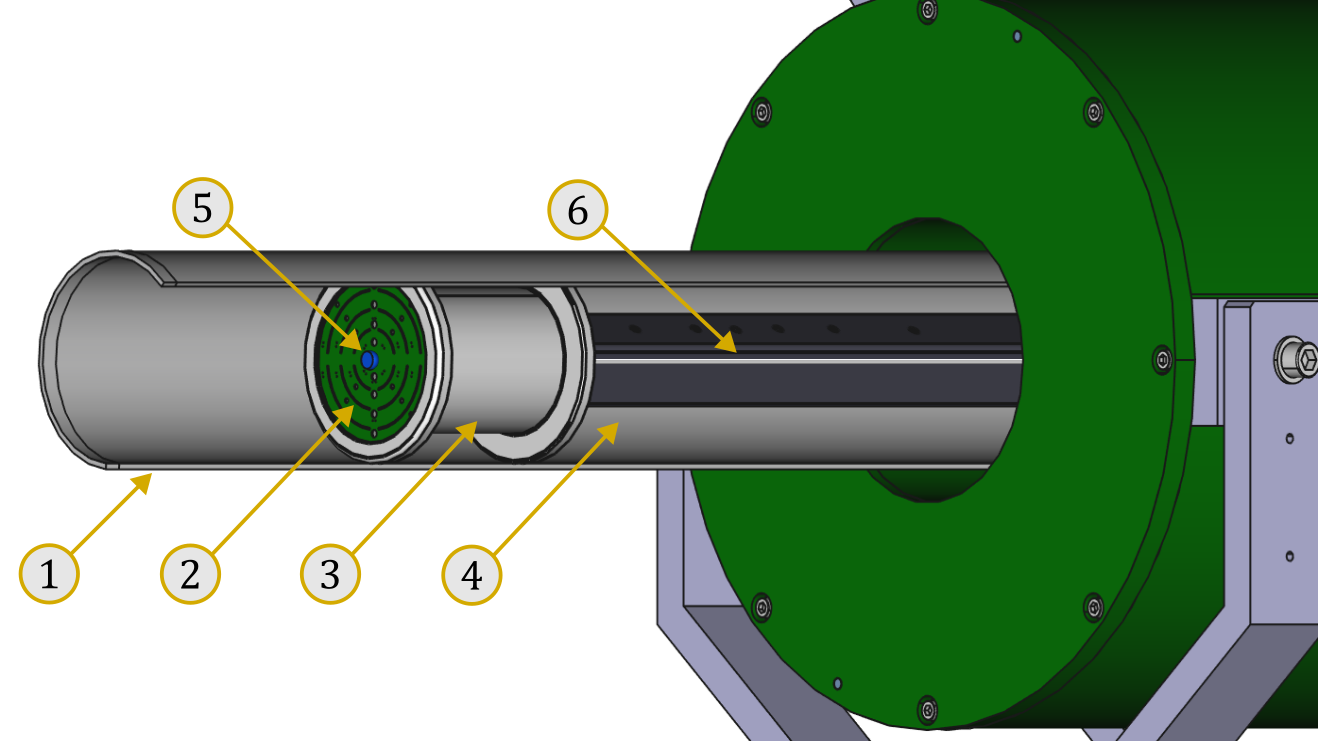
\includegraphics[width=0.7\textwidth]{figs/elena}
    \caption{The fluxmeter assembly going through a solenoid magnet. \\
    1. Guiding Tube, 2. Fluxmeter PCB, 3. PCB Sledge, 4. Supporting arm, 
    5. Laser Reflector, 6. Encoder Wire.
    Magnet model courtesy {AD_MLNAF0001}.}
    \label{fig:elena}
\end{figure}

To move the PCB through the magnet aperture, a support assembly was made as
seen in figure \ref{fig:elena}. The coil cables are run through the supporting
arm, which is also used to push and pull the fluxmeter through the tube. A 
wire is connected to the PCB sledge on one end, and spooled up around
a rotating encoder on the other end. In the middle of the PCB, a 
reflector is mounted for the laser tracker.

\section{PCB printed coils}
The coil PCB has 21 different coils.
These coils are in the shapes of disks or annulus segments.
A render of the pcb can be seen in figure
\ref{fig:pcb}. The disks are denoted $D_l$ and the 
annulus segments by $Q_{q, l}$ where $l$ is the radial layer and 
$q$ is the quadrant, as seen in figure \ref{fig:nomenclature}.

\begin{figure}[!h]
    \centering
    \begin{subfigure}[b]{0.5\linewidth}
        \centering
        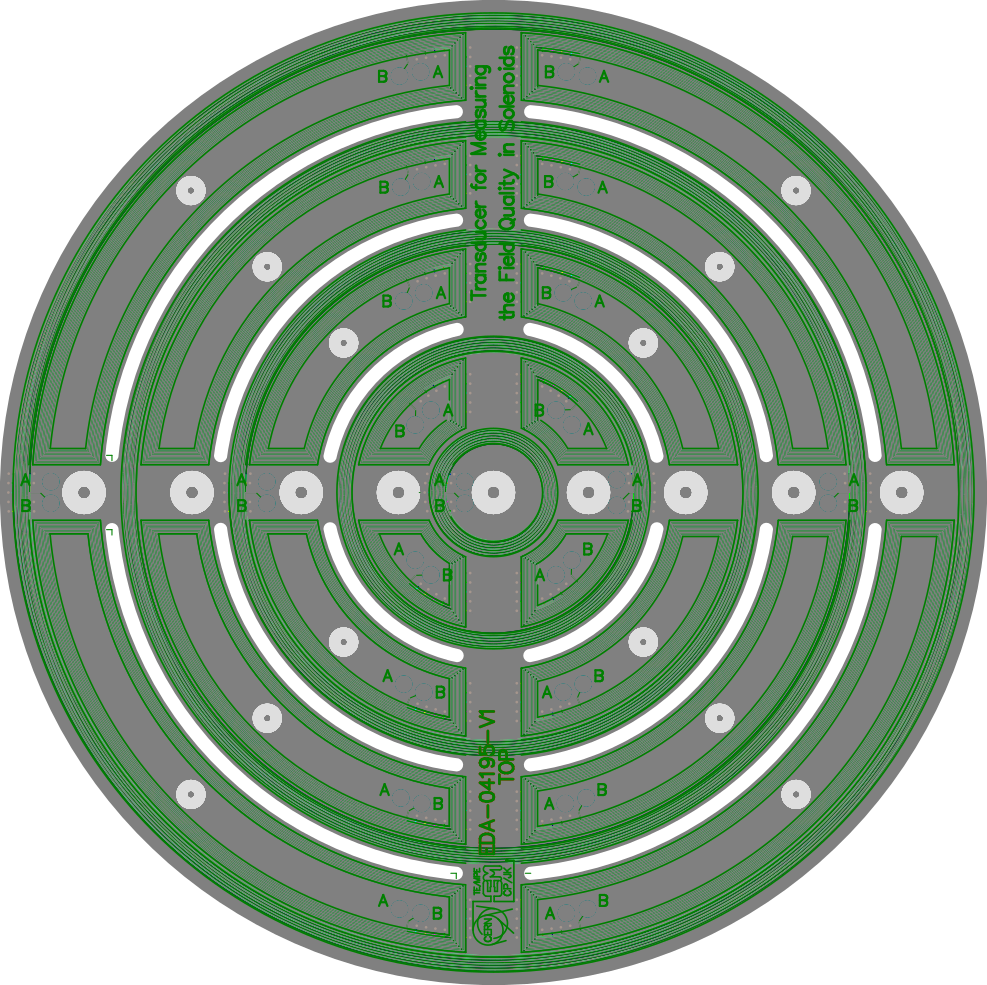
\includegraphics[width=0.8\linewidth]{figs/pcb}
        \caption{The fluxmeter PCB.}
        \label{fig:pcb}
    \end{subfigure}
    \hfill
    \begin{subfigure}[b]{0.4\linewidth}
        \centering
        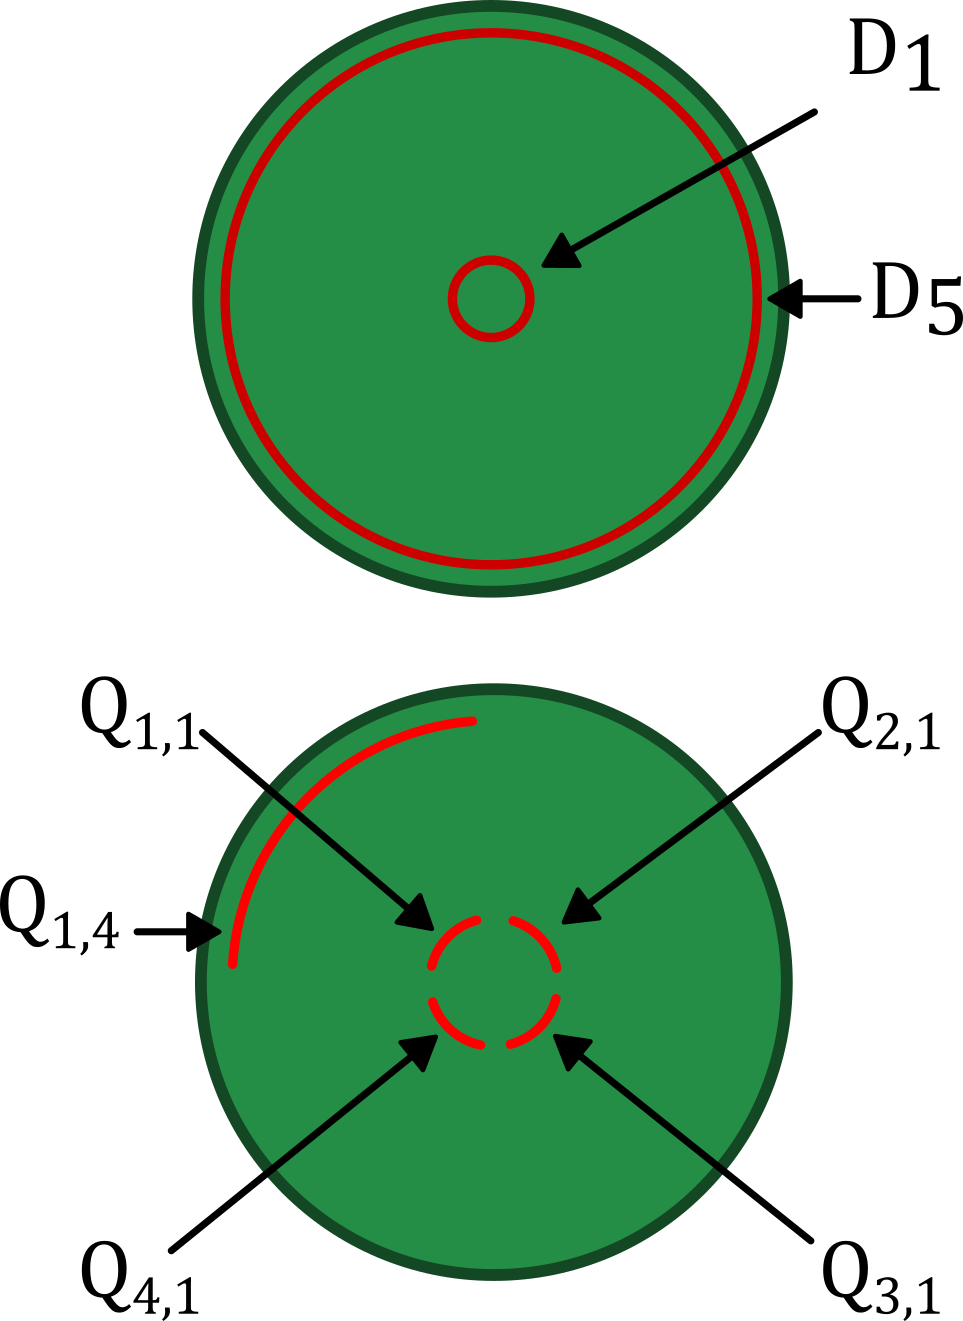
\includegraphics[width=0.8\linewidth]{figs/nomenclature.png}
        \caption{Nomenclature of the PCB coils.}
        \label{fig:nomenclature}
    \end{subfigure}
    \caption{}
\end{figure}

During measurements, the magnet is magnetized with a constant current.
As the coils move through the magnet, a voltage is induced according 
to Faradays Law, equation \ref{eq:faraday}. Although the field is 
static, since the fluxmeter is moving it will still see a delta
flux with respect to time.

\section{Geometric Laser Measurements}
The laser tracker works by shooting a laser at a reflector, and then
measuring the time of flight. The accuracy depends on the reflector
type and measurement time, but an upper limit of 
0.2 mm is a reasonable estimate according to the
specifications of both the reflectors and laser tracker
used. \cite{leica_manual}. 

Firstly, scans were done of a network of reflectors around the 
room. These points were then used as a baseline to locate the
laser tracker at the start of each measurement campaign, or when
the laser tracker needed to be moved. A cluster of points were
taken of the magnet itself. These points
were then fitted to a cylinder. Using a 3D model of the
solenoid, a coordinate system could be constructed
with its origin at the geometric center of the magnet.
Furthermore, two planes were constructed at the positions
of the clamps holding the fluxmeter guiding tube. The 
positions of these clamps could accurately be moved in
both lateral dimensions using precision dials. In effect,
the tube has two anchor points that can be moved along
the aforementioned planes, so that it can be aligned (or misaligned)
as desired.

\begin{figure}[!h]
    \centering
    \includegraphics[width=0.7\textwidth]{figs/3Dscan}
    \caption{3D scans of the measurement assembly.
    1: Laser Tracker, 2: 3D scan of the solenoid, 
    3: Network Point, 4: Tube clamp positioning planes.
    3D scans fitted using Spatial Analyzer \cite{spatial_analyzer}.}
    \label{fig:3dscan}
\end{figure}

\section{Positional Encoder}
The positional encoder is a rotating encoder connected to a wire spool.
As the fluxmeter moves through the the magnet, it pulls on the wire,
making the rotating encoder move.
\section{Fast Digital Integrators}
\section{The Measurement Assembly}